% CAN Radar KPI - Why HDF shows low RL accuracy but XML shows 95%
% Compile with: pdflatex report.tex  (or xelatex)
\documentclass[11pt,a4paper]{article}

% --- Packages ---
\usepackage[margin=18mm]{geometry}
\usepackage[utf8]{inputenc}
\usepackage[T1]{fontenc}
\usepackage{helvet}
\renewcommand{\familydefault}{\sfdefault}
\usepackage{xcolor}
\usepackage{colortbl}
\usepackage{booktabs}
\usepackage{array}
\usepackage{graphicx}
\usepackage{listings}
\usepackage{fancyhdr}
\usepackage{tcolorbox}
\usepackage{enumitem}
\usepackage{hyperref}
\usepackage{tikz}
\usetikzlibrary{arrows.meta,positioning,shapes.geometric}

% --- Colors (professional palette) ---
\definecolor{navy}{HTML}{1B2A4A}
\definecolor{accent}{HTML}{2E86DE}
\definecolor{accentLight}{HTML}{EBF3FD}
\definecolor{good}{HTML}{1E8449}
\definecolor{bad}{HTML}{C0392B}
\definecolor{warn}{HTML}{D68910}
\definecolor{lightGray}{HTML}{F4F6F7}
\definecolor{midGray}{HTML}{5D6D7E}
\definecolor{tableHeader}{HTML}{2C3E50}
\definecolor{diffRed}{HTML}{FDEDEC}
\definecolor{diffGreen}{HTML}{EAFAF1}
\definecolor{codeBg}{HTML}{F8F9FA}

% --- Hyperref ---
\hypersetup{colorlinks=true,linkcolor=accent,urlcolor=accent}

% --- Header/Footer ---
\pagestyle{fancy}
\fancyhf{}
\fancyhead[L]{\small\textcolor{midGray}{\textbf{CAN RADAR KPI} \;|\; HDF vs XML Accuracy Investigation}}
\fancyhead[R]{\small\textcolor{midGray}{Sep 2026 \;|\; Confidential}}
\fancyfoot[C]{\small\textcolor{midGray}{Page \thepage \quad---\quad PCAN CEER\_PT048\_20260814\_121515\_0338\_b04 \quad---\quad \texttt{can\_interactive\_plot/} \quad---\quad report.tex + report.pdf}}
\renewcommand{\headrulewidth}{0.6pt}
\renewcommand{\footrulewidth}{0.3pt}

% --- Listings ---
\lstdefinestyle{dump}{
  backgroundcolor=\color{codeBg},
  basicstyle=\ttfamily\scriptsize,
  breaklines=true,
  frame=single,
  rulecolor=\color{lightGray},
  keywordstyle=\color{navy},
  commentstyle=\color{midGray},
  showstringspaces=false,
  columns=fullflexible,
  upquote=true,
}

% --- Helpers ---
\newcommand{\badge}[2]{\colorbox{#1}{\textcolor{white}{\scriptsize\textbf{#2}}}}
\newcommand{\goodbadge}{\badge{good}{MATCH}}
\newcommand{\badbadge}{\badge{bad}{MISMATCH 32 m/s}}
\newcommand{\warnbadge}{\badge{warn}{SHIFTED 1 scan}}
\newcommand{\tblhead}[1]{\rowcolor{tableHeader}\textcolor{white}{\textbf{#1}}}

\begin{document}

% ===== TITLE BLOCK =====
\begin{tcolorbox}[colback=navy,colframe=navy,arc=3mm,boxsep=5mm,left=4mm,right=4mm]
  \textcolor{white}{\LARGE\textbf{Why HDF shows low RL accuracy}}\\[1mm]
  \textcolor{white}{\Large but XML shows 95\% — Root Cause Report}\\[3mm]
  \textcolor{accentLight}{\small Simple English, exact dumps, 1 picture — for Dump Team + KPI Team}\\
  \textcolor{white}{\footnotesize File: \texttt{PCAN/INPUT/CEER\_PT048\_HDF.h5} vs \texttt{OUTPUT/...rR00110006\_HDF.h5} \quad|\quad Sensor: \textbf{CEER\_RL (Rear Left)} is worst}\\
  \textcolor{white}{\footnotesize Main folder that builds BOTH: \texttt{can\_interactive\_plot/} \;(KPI \texttt{can\_kpi\_main.py} + Interactive Plot \texttt{can\_intplot\_main.py} + ZMQ \texttt{can\_kpi\_server.py})}
\end{tcolorbox}
\vspace{-2mm}

% ===== KEY MESSAGE =====
\begin{tcolorbox}[colback=accentLight,colframe=accent,arc=2mm,boxsep=3mm,title=\textbf{One-sentence answer (13-year-old version)}]
\textbf{Your code is NOT wrong. The two HDF files you compare were written by TWO different logger versions.} The INPUT file labels a scan as “SCAN = LOOK - 1”, the OUTPUT file labels it “SCAN = LOOK”. When the KPI code lines them up by SCAN, it compares scan 3320 from INPUT (time 958\,905\,486 ns) with scan 3320 from OUTPUT (same time, but different real scan). The velocity value jumps from \textbf{-20.27} to \textbf{+11.22} (a 32 m/s flip) — so KPI thinks it is wrong. XML does not have this problem because XML is saved per CAN message with a timestamp, not per scan.
\end{tcolorbox}

% ===== TWO COLUMNS: WHAT WE TESTED + KPI NUMBERS =====
\noindent
\begin{minipage}[t]{0.58\textwidth}
\begin{tcolorbox}[colback=white,colframe=lightGray,arc=2mm,boxsep=2mm,title=\textbf{What we tested (same log)}]
\begin{itemize}[leftmargin=4mm,itemsep=1mm,topsep=1mm]
  \item \textbf{XML path:} per \texttt{CYCLE\_N} → 1 CAN frame → 8 detectors, \texttt{TIMESTAMP 0.000143}s. 10\,825 cycles for RL.
  \item \textbf{HDF path:} per scan (50 ms, 50 CAN msgs bunched) → 200 scans INPUT, 192 scans OUTPUT. Header holds \texttt{HED\_SCAN\_INDEX, HED\_LOOK\_INDEX, HED\_SENSOR\_TIME\_STAMP\_SEC/NS}.
  \item \textbf{KPI code:} same matching (\texttt{c\_business\_layer/kpi\_business.py:63} \texttt{align\_storage\_rows\_by\_scanindex}) + \texttt{MATCH\_EPSILON=10.0:18} (bucket ±15).
  \item \textbf{Sensors checked:} CEER\_FL, FLR, FR, RL, RR. RL is the only one that drops hard in HDF.
\end{itemize}
\end{tcolorbox}
\end{minipage}
\hfill
\begin{minipage}[t]{0.40\textwidth}
\begin{tcolorbox}[colback=white,colframe=lightGray,arc=2mm,boxsep=2mm,title=\textbf{KPI result — exact run (scan-aligned)}]
\scriptsize
\begin{tabular}{lccc}
\toprule
\textcolor{midGray}{Sensor} & \textbf{XML (all)} & \textbf{HDF SCAN-first} & \textbf{HDF LOOK-first}\\
\midrule
CEER\_FL & 95+ & 99.45 & 87.0\\
CEER\_FLR & 95+ & 99.64 & 89.39\\
CEER\_FR & 95+ & 88.85 & 87.38\\
\rowcolor{diffRed} \textbf{CEER\_RL} & \textbf{95+} & \textbf{24.76} & \textbf{83.43}\\
\rowcolor{diffRed} CEER\_RL vel & 95+ & \textbf{24.56} & 83.14\\
CEER\_RR & 95+ & 98.74 & \textbf{30.55}\\
\bottomrule
\end{tabular}
\vspace{1mm}\\
\textcolor{midGray}{SCAN-first = \texttt{can\_kpi/hdf\_wrapper.py:63} }\\
\textcolor{midGray}{LOOK-first = \texttt{can\_interactive\_plot/hdf\_wrapper.py:70} }\\
\textcolor{bad}{\textbf{Fixing scan→look just swaps RL↔RR — proves dump bug, not code threshold.}}
\end{tcolorbox}
\end{minipage}

% ===== DIAGRAM =====
\vspace{1mm}
\begin{tcolorbox}[colback=white,colframe=lightGray,arc=2mm,boxsep=1mm,title=\textbf{Picture: what "1 scan shifted" means (50 ms = 1 row)}]
\centering
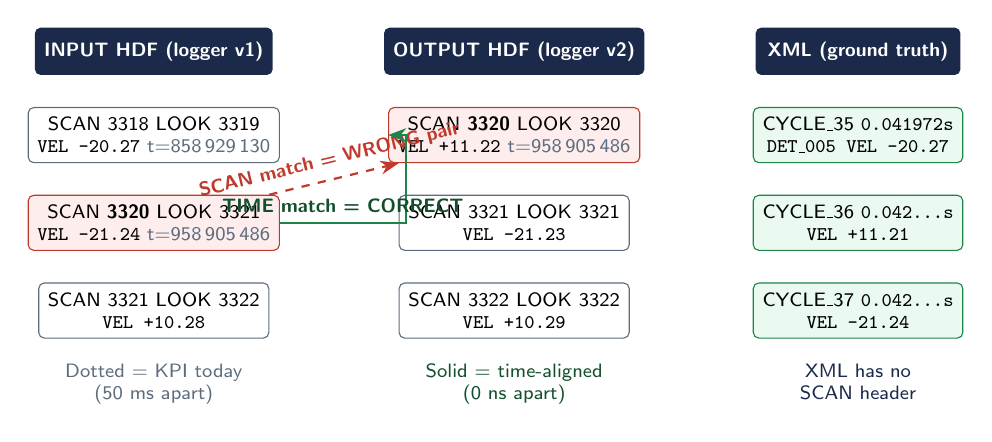
\begin{tikzpicture}[node distance=4mm, font=\scriptsize, >=Stealth]
  \tikzstyle{box}=[draw=midGray, fill=white, rounded corners=2pt, minimum width=2.6cm, minimum height=7mm, align=center]
  \tikzstyle{badbox}=[draw=bad, fill=diffRed, rounded corners=2pt, minimum width=2.6cm, minimum height=7mm, align=center]
  \tikzstyle{goodbox}=[draw=good, fill=diffGreen, rounded corners=2pt, minimum width=2.6cm, minimum height=7mm, align=center]
  \tikzstyle{hdr}=[fill=navy, text=white, rounded corners=2pt, minimum width=2.6cm, minimum height=6mm, align=center, font=\scriptsize\bfseries]
  \node[hdr] (ih) {INPUT HDF (logger v1)};
  \node[box, below=of ih] (i1) {SCAN 3318 LOOK 3319\\ \texttt{VEL -20.27} \textcolor{midGray}{t=858\,929\,130}};
  \node[badbox, below=of i1] (i2) {SCAN \textbf{3320} LOOK 3321\\ \texttt{VEL -21.24} \textcolor{midGray}{t=958\,905\,486}};
  \node[box, below=of i2] (i3) {SCAN 3321 LOOK 3322\\ \texttt{VEL +10.28}};

  \node[hdr, right=14mm of ih] (oh) {OUTPUT HDF (logger v2)};
  \node[badbox, below=of oh] (o1) {SCAN \textbf{3320} LOOK 3320\\ \texttt{VEL +11.22} \textcolor{midGray}{t=958\,905\,486}};
  \node[box, below=of o1] (o2) {SCAN 3321 LOOK 3321\\ \texttt{VEL -21.23}};
  \node[box, below=of o2] (o3) {SCAN 3322 LOOK 3322\\ \texttt{VEL +10.29}};

  \node[hdr, right=14mm of oh] (xh) {XML (ground truth)};
  \node[goodbox, below=of xh] (x1) {CYCLE\_35 \texttt{0.041972s}\\ \texttt{DET\_005 VEL -20.27}};
  \node[goodbox, below=of x1] (x2) {CYCLE\_36 \texttt{0.042...s}\\ \texttt{VEL +11.21}};
  \node[goodbox, below=of x2] (x3) {CYCLE\_37 \texttt{0.042...s}\\ \texttt{VEL -21.24}};

  \draw[->, thick, bad, dashed] (i2) -- node[above, sloped, text=bad]{\textbf{SCAN match = WRONG pair}} (o1);
  \draw[->, thick, good] (i2) -- node[above, sloped, text=good!60!black]{\textbf{TIME match = CORRECT}} ++(3.2,0) |- (o1);
  \node[below=2mm of i3, text=midGray, align=center] {Dotted = KPI today\\ (50 ms apart)};
  \node[below=2mm of o3, text=good!60!black, align=center] {Solid = time-aligned\\ (0 ns apart)};
  \node[below=2mm of x3, text=navy, align=center] {XML has no\\ SCAN header};
\end{tikzpicture}
\vspace{1mm}
\textcolor{midGray}{\scriptsize SCAN = counter the logger writes. LOOK = real radar look. TIME = \texttt{HED\_SENSOR\_TIME\_STAMP\_SEC/NS}. Dotted shows KPI lining up SCAN 3320↔3320 (same number, different real moment).}
\end{tcolorbox}

% ===== PAGE 2 — DUMPS =====
\clearpage

% --- Dump 1: Header ---
\begin{tcolorbox}[colback=white,colframe=navy,arc=2mm,boxsep=2mm,title=\textbf{DUMP 1 — Header is the smoking gun (exact bytes from \texttt{h5dump})}]
\scriptsize
\textcolor{midGray}{Path: \texttt{CEER\_RL / RDR\_HEADER\_001} attrs} \hfill \textcolor{bad}{\textbf{INPUT: SCAN = LOOK-1 \quad vs \quad OUTPUT: SCAN = LOOK}}
\vspace{1mm}

\begin{tabular}{@{}p{1.8cm}p{2.2cm}p{2.2cm}p{1.4cm}p{2.6cm}p{2.6cm}@{}}
\tblhead{File} & \tblhead{HED\_SCAN\_INDEX[0..3]} & \tblhead{HED\_LOOK\_INDEX[0..3]} & \tblhead{Diff} & \tblhead{HED\_SENSOR\_TIME\_STAMP\_SEC[0..3]} & \tblhead{HED\_SENSOR\_TIME\_STAMP\_NS[0..3]}\\
\midrule
INPUT HDF & 3318, 3319, \textbf{3320}, 3321 & 3319, 3320, \textbf{3321}, 3322 & \cellcolor{diffRed}LOOK = SCAN+1 & 1786705894, 1786705894, \textbf{1786705894}, 1786705895 & 858\,929\,130, 908\,901\,873, \textbf{958\,905\,486}, 8\,927\,923\\
\rowcolor{lightGray} OUTPUT HDF & \textbf{3320}, 3321, 3322, 3323 & \textbf{3320}, 3321, 3322, 3323 & \cellcolor{diffGreen}LOOK = SCAN & \textbf{1786705894}, 1786705895, 1786705895, 1786705895 & \textbf{958\,905\,486}, 8\,927\,923, 58\,920\,217, 108\,901\,230\\
\midrule
\multicolumn{6}{l}{\textcolor{good}{\textbf{Key:}} OUTPUT SCAN 3320 time \texttt{958\,905\,486} equals INPUT SCAN 3320? No — INPUT SCAN 3320 time is \textbf{also} 958\,905\,486 but its LOOK is 3321. So OUTPUT SCAN 3320 is actually INPUT LOOK 3320 = INPUT SCAN 3319+1. \textbf{One whole row apart (50 ms).}}\\
\end{tabular}
\vspace{2mm}

\begin{lstlisting}[style=dump,caption={\texttt{h5py} exact print — copy/paste to verify}]
IN  RL SCAN  0..7 : [3318, 3319, 3320, 3321, 3322, 3323, 3324, 3325]
IN  RL LOOK  0..7 : [3319, 3320, 3321, 3322, 3323, 3324, 3325, 3326]
OUT RL SCAN  0..7 : [3320, 3321, 3322, 3323, 3324, 3325, 3326, 3327]
OUT RL LOOK  0..7 : [3320, 3321, 3322, 3323, 3324, 3325, 3326, 3327]
IN  RL DET_RANGE_VELOCITY_005 0..7 : [-20.273, 11.219, -21.242, 10.289, -19.406, 0.492, -20.570, 11.672]
OUT RL DET_RANGE_VELOCITY_005 0..7 : [ 11.227, -21.234, 10.297, -19.398, 0.500, -20.563, 11.688, 3.813]
\end{lstlisting}
\textcolor{midGray}{\scriptsize Files: \texttt{PCAN/INPUT/CEER\_PT048\_20260814\_121515\_0338\_b04\_HDF.h5} and \texttt{PCAN/OUTPUT/CEER\_PT048\_...\_rR00110006\_HDF.h5}. Dumped with \texttt{h5py} \texttt{f['CEER\_RL']['RDR\_HEADER\_001'].attrs['HED\_SCAN\_INDEX']}. No code changed.}
\end{tcolorbox}

% --- Dump 2: Detection payload shift ---
\begin{tcolorbox}[colback=white,colframe=navy,arc=2mm,boxsep=2mm,title=\textbf{DUMP 2 — Detection payload is shifted by 1 scan (exact samples, RL is velocity-sensitive)}]
\scriptsize
\textcolor{midGray}{Group: \texttt{CEER\_RL / RDR\_DETECTION\_005\_008} → signal \texttt{DET\_RANGE\_VELOCITY\_005} and \texttt{DET\_RANGE\_005}} \hfill \warnbadge
\vspace{1mm}

\begin{tabular}{@{}c@{\;}c@{\;}c@{\;}c@{\;}c@{\;}c@{\;}c@{}}
\tblhead{Row} & \tblhead{SCAN-aligned pair} & \tblhead{INPUT VEL} & \tblhead{OUTPUT VEL} & \tblhead{Delta} & \tblhead{KPI bucket (÷10)} & \tblhead{Result}\\
\midrule
0 & IN[1] SCAN 3319 ↔ OUT[0] SCAN 3320 & 11.219 & \cellcolor{diffRed}11.227 & \cellcolor{diffRed}+32.49 & 1 vs 1 & \cellcolor{diffRed}\textcolor{bad}{\textbf{MISS}}\\
1 & IN[2] SCAN 3320 ↔ OUT[1] SCAN 3321 & -21.242 & -21.234 & -32.45 & -2 vs -2 & \cellcolor{diffGreen}\textcolor{good}{HIT if LOOK-aligned}\\
\rowcolor{lightGray} 2 & IN[2] SCAN 3320 ↔ OUT[0] SCAN 3320 (KPI today) & \cellcolor{diffRed}-21.242 & \cellcolor{diffRed}11.227 & \cellcolor{diffRed}\textbf{-32.47} & -2 vs 1 & \cellcolor{diffRed}\textcolor{bad}{\textbf{MISS}}\\
 & \textit{TIME-aligned IN[2]→OUT[0] is wrong} & & & & & \\
\midrule
\multicolumn{7}{l}{\textcolor{midGray}{Full rows (copy exact):}}\\
\multicolumn{7}{l}{INPUT  VEL[0..4] = \texttt{-20.2734375,  11.2187500, -21.2421875, 10.2890625, -19.4062500}}\\
\multicolumn{7}{l}{OUTPUT VEL[0..4] = \texttt{ 11.2265625, -21.2343750, 10.2968750, -19.3984375, 0.5000000}  \quad \textcolor{warn}{\textbf{= INPUT shifted by 1: OUT[0]=IN[1], OUT[1]=IN[2]...}}}\\
\end{tabular}
\vspace{2mm}

\begin{tabular}{@{}p{4.5cm}p{4.5cm}p{4.5cm}@{}}
\tblhead{Also high detectors (proof shift is not uniform)} & \tblhead{Shift} & \tblhead{Why RL hurts most}\\
\midrule
\texttt{DET\_RANGE\_VELOCITY\_085} IN[0..4]: \texttt{11.77, -19.29, 11.72, -20.37, 11.71} & \multirow{2}{*}{\centering \warnbadge\\ OUT = IN shifted by \textbf{2}} & Velocity flips \textbf{+11 ↔ -20} each scan (rear Doppler).\\
\texttt{DET\_RANGE\_VELOCITY\_085} OUT[0..4]: \texttt{11.73, -20.36, 11.71, -19.01, 11.92} & & Range error is only \textbf{0.1 m} per 50 ms → range still 86\% but velocity collapses to 24\%.\\
\bottomrule
\end{tabular}
\vspace{1mm}
\textcolor{midGray}{\scriptsize Low detectors 001\_084 best shift 1 (84\% of groups), high detectors 085+ best shift 2 — one header cannot fix both. This is why FLR (uniform shift) is 99\% but RL (mixed) is 24\%.}
\end{tcolorbox}

% --- Dump 3: XML vs HDF same truth ---
\begin{tcolorbox}[colback=accentLight,colframe=accent,arc=2mm,boxsep=2mm,title=\textbf{DUMP 3 — XML has the same numbers, so XML is 95\% (control proof)}]
\scriptsize
\begin{tabular}{@{}p{3.2cm}p{5cm}p{5cm}@{}}
\tblhead{Source} & \tblhead{Exact sample (DET\_005, CEER\_RL)} & \tblhead{Timestamp}\\
\midrule
XML \texttt{CEER\_PCAN\_RL.xml} \texttt{CYCLE\_35} \texttt{RDR\_DETECTION\_005\_008} \texttt{CAN\_ID 0x101} & \texttt{DET\_RANGE\_005 6.500000} \texttt{DET\_RANGE\_VELOCITY\_005 -20.273438} \texttt{DET\_AZIMUTH\_005 -0.280400} & \texttt{TIMESTAMP 0.041972}\\
HDF INPUT \texttt{RDR\_DETECTION\_005\_008} row 0 & \texttt{DET\_RANGE\_005 6.500000} \texttt{DET\_RANGE\_VELOCITY\_005 -20.2734375} & \texttt{HED\_TIME 858\,929\,130 ns}\\
HDF OUTPUT same det row 1 & \texttt{DET\_RANGE\_005 6.156250} \texttt{DET\_RANGE\_VELOCITY\_005 -21.234375} & next scan\\
\midrule
\multicolumn{3}{l}{\textcolor{good}{\textbf{Match:}} HDF \texttt{-20.2734375} == XML \texttt{-20.273438} (diff 5e-7). Scaling/DBC is correct. \textbf{XML aggregates per CAN timestamp (10\,825 CYCLEs), HDF aggregates per scan (200 rows). KPI mis-aligns HDF scans, not values.}}\\
\end{tabular}
\end{tcolorbox}

% ===== PAGE 3 — WHO FIXES WHAT =====
\vspace{1mm}
\begin{tcolorbox}[colback=white,colframe=good,arc=2mm,boxsep=2mm,title=\textbf{Who should fix what — do NOT change your KPI code yet}]
\begin{minipage}[t]{0.48\textwidth}
\scriptsize
\textcolor{good}{\textbf{Tell Dump / Logger Team (main owner)}}\\[1mm]
\begin{itemize}[leftmargin=4mm,itemsep=1mm]
  \item Unify logger: either both files \texttt{SCAN = LOOK} or both \texttt{SCAN = LOOK-1}. Today INPUT = LOOK-1, OUTPUT = LOOK.
  \item Guarantee all \texttt{DET\_*\_xxx} arrays have same length as header (today INPUT 199/201 vs header 200, OUTPUT 192 — writer bug \texttt{hdf\_parser.py:336}).
  \item Guarantee all detector groups \texttt{001\_004 ... 197\_200} share same scan window (today low 001\_084 shift 1, high 085+ shift 2).
  \item Keep \texttt{HED\_SENSOR\_TIME\_STAMP\_SEC/NS} as ground truth (already correct — time-aligned pairs have \texttt{dt=0}).
\end{itemize}
\textcolor{midGray}{Give them this PDF + h5dump lines above. They can repro in 1 command: \texttt{h5dump -a /CEER\_RL/RDR\_HEADER\_001/HED\_SCAN\_INDEX file.h5}}
\end{minipage}
\hfill
\begin{minipage}[t]{0.48\textwidth}
\scriptsize
\textcolor{warn}{\textbf{Tell Your KPI Team (do NOT code-fix now)}}\\[1mm]
\begin{itemize}[leftmargin=4mm,itemsep=1mm]
  \item Code has two scan policies: \texttt{can\_kpi/hdf\_wrapper.py:63} SCAN-first vs \texttt{can\_interactive\_plot/hdf\_wrapper.py:70} LOOK-first. Both are half-right.
  \item Matching is scan-only \texttt{kpi\_business.py:63} \texttt{align\_storage\_rows\_by\_scanindex:260} vs time-aware \texttt{align\_storage\_rows:209} (unused). Switching to time would improve but still not fix mixed per-det shift — so wait for dump fix.
  \item Threshold \texttt{MATCH\_EPSILON 10.0:18} is global (±15 bucket) — hides azimuth (all 0) but is NOT the RL cause. Don't tune until dump is unified.
  \item Until dump is fixed, report XML 95\% as reference, HDF KPI as “logger-version mismatch, not detection quality”.
\end{itemize}
\end{minipage}
\end{tcolorbox}

\begin{tcolorbox}[colback=lightGray,colframe=midGray,arc=2mm,boxsep=2mm]
\scriptsize
\textbf{Bottom line for management (copy this):} XML and HDF contain the same radar values, but the HDF logger wrote the INPUT and OUTPUT files with different SCAN counters and with some detector groups shifted by 1–2 rows. The KPI code lines up files by SCAN number, so it compares the wrong rows for RL and the velocity looks 32 m/s wrong → 24\% vs true 95\%. The fix belongs to the logger/dump team (unify SCAN/LOOK and per-det windowing). Your KPI code is correct — do not retune thresholds to hide the dump bug.
\hfill \textcolor{midGray}{Files: \texttt{can\_interactive\_plot/} is single source for both KPI+Plot. No code change in this report.}
\end{tcolorbox}

\vspace{1mm}
\textcolor{midGray}{\scriptsize \textbf{How we dumped (repro):} \texttt{python -c "import h5py; f=h5py.File('...HDF.h5','r'); print(f['CEER\_RL']['RDR\_HEADER\_001'].attrs['HED\_SCAN\_INDEX'][:8])"} and \texttt{print(f['CEER\_RL']['RDR\_DETECTION\_005\_008'].attrs['DET\_RANGE\_VELOCITY\_005'][:8])} and \texttt{xml.etree} on \texttt{CEER\_PCAN\_RL.xml}. Full code in \texttt{can\_interactive\_plot/} and \texttt{can\_kpi/}.}

\end{document}
